\section{Complex pipelining}

Pipelining complexity increases significantly when aiming for high performance, especially in the presence of:
\begin{itemize}
    \item Long latency or partially pipelined floating-point units.
    \item Multiple function and memory units.
    \item Memory systems with variable access time.
    \item Precise exception handling.
\end{itemize}
One potential solution is the complex in order pipeline:
\begin{itemize}
    \item Introduce a delay in the write-back stage to ensure all operations have the same latency to the write-back stage.
    \item Avoid over subscription of write ports, allowing for one instruction to enter and one instruction to exit every cycle.
    \item Enforce in-order instruction commitment, which simplifies the implementation of precise exception handling.
\end{itemize}
\begin{figure}[H]
    \centering
    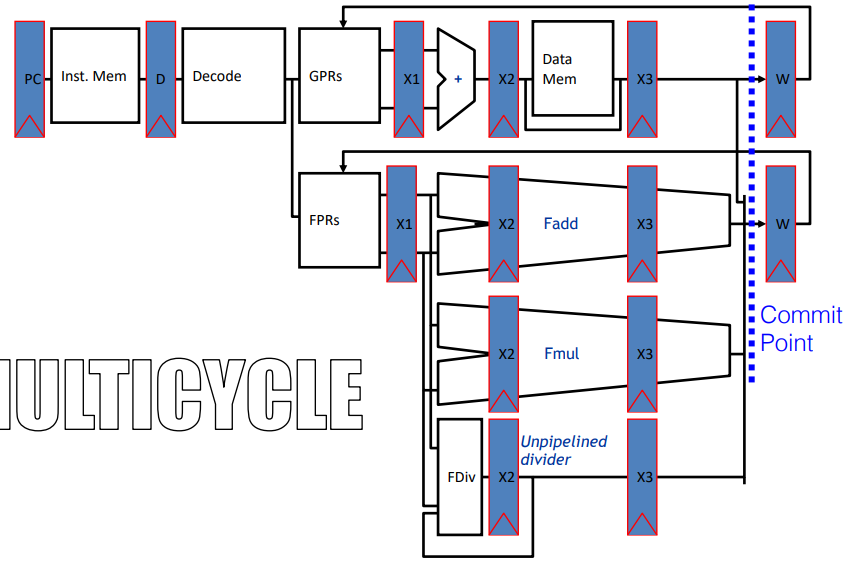
\includegraphics[width=0.3\linewidth]{images/ciop.png}
    \caption{Complex in order pipeline}
\end{figure}

\paragraph*{Issues}
Structural conflicts arise during the execution stage if certain Floating Point Units (FPU) or memory units are not pipelined, causing them to take longer than one cycle.
There are also structural conflicts at the write-back stage because different functional units may have variable latencies.
Additionally, out-of-order write hazards occur due to the variable latencies of different functional units.